\documentclass[11pt,b5paper,onecolumn,titlepage,openright,twoside,final]{book}
\usepackage{pdfpages}
\usepackage{dcolumn}
\usepackage{graphicx}
\usepackage{amsmath}
% \usepackage{bm}
\usepackage{epigraph}
\usepackage{rotating}
\usepackage[nottoc,notlof,notlot]{tocbibind}
\usepackage{times}
\usepackage{fancyhdr}
\usepackage{lipsum}
\usepackage[Sonny]{fncychap}
\usepackage{epstopdf}
\usepackage{color}
\usepackage{fontspec}
\usepackage{unicode-math}
\setmainfont[Ligatures=TeX]{TeX Gyre Pagella}
\usepackage[colorlinks=false,xetex,bookmarks=false]{hyperref} %Internal links.
\usepackage[capitalize]{cleveref} %Automatic referencing (with capital letters)
\usepackage[numbers, sort&compress]{natbib}
\begin{document}

\newcommand{\bv}[1]{\mathbfup{#1}}
\newcommand{\bvh}[1]{\hat{\bv{#1}}}
\newcommand{\dd}[0]{\text{d}}
\definecolor{Red}{rgb}{1,0,0}
\definecolor{Blu}{rgb}{0,0,01}
\definecolor{Green}{rgb}{0,1,0}
\definecolor{Purple}{rgb}{0.5,0,0.5}
\newcommand{\red}{\color{Red}}
\newcommand{\blu}{\color{Blu}}
\newcommand{\green}{\color{Green}}
\newcommand{\purple}{\color{Purple}}

\pagestyle{empty}
\frontmatter
% \title{Monte-Carlo studies of\\ multi-component Ginzburg-Landau theories with competing interactions}
% \author{Peder Notto Galteland}
% \date{\today}
% \maketitle
\chapter*{Abstract}
\chapter*{Abstract}\noindent
This is a \textsc{latex} template intended for academic theses, and was put together by \href{https://github.com/jabirali}{Jabir Ali Ouassou} while preparing his PhD dissertation.
The template itself is released under a Creative Commons Attribution licence (\href{https://creativecommons.org/licenses/by/4.0/}{\textsc{cc by 4.0}}).
This basically means that you are free to use the template for any purpose as long as you give appropriate credit.

The template bundles the \href{https://github.com/libertinus-fonts/libertinus}{Libertinus fonts}, which is used for all regular text and mathematics, and the \href{https://ctan.org/tex-archive/fonts/urw/classico}{\textsc{urw} classico} fonts, which are used for chapter and section headings.
The former is available under the Open Font Licence (\textsc{sil ofl 1.1}), and is free for both private and commercial use.
The latter is available under the Aladdin Free Public Licence (\textsc{afpl}), and is only free for non-commercial use.
If commercial use is of importance, a suitable replacement for \textsc{urw} classico would be the Libertinus Sans fonts, which are also bundled with the template.

Note that this template relies on \textsc{lualatex} for \eg font customization, and on \textsc{bibtex} for reference handling.
For command-line users, the easiest way to compile the document is to run \texttt{latexmk -lualatex thesis.tex}.
If using an \textsc{ide}, please check the program settings for how to enable compilation with \textsc{lualatex} and \textsc{bibtex}.
The template is based on the \textsc{koma-script} book class (\texttt{scrbook}), so for further customization of the template, please check out \href{https://ctan.org/pkg/koma-script}{their documentation}.

The template does not include a title page.
This is because the style requirements typically varies between universities, and many institutions will anyway autogenerate a titlepage upon thesis submission.


\chapter*{Preface}
\chapter*{Preface}\noindent

This thesis is submitted in partial satisfaction of the requirements of the degree Philosophiae Doctor (PhD) at the
Norwegian University of Science and Technology, in Trondheim Norway.

The work that this thesis presents started in September 2015 and ended in early spring 2021 at the
\href{https://www.ntnu.edu/quspin/center-for-quantum-spintronics}{Center for Quantum Spintronics (\textsc{QuSpin})}, \textsc{NTNU}. During this time, one
year of accumulated time was dedicated to teaching duties at the Department of Physics, and half a year
was devoted to completion of courses (30 ECTS) as pr. the requirements of the degree.
The research was supervised by
Prof. Asle Sudb{\o} as main supervisor, and Prof. Jacob Linder as co-supervisor.

Computation-time was granted at the \textsc{Vilje} and \textsc{Fram} supercomputers through the UNINETT $\int$igma$2$ e-infrastructure. The code was written in
the \href{https://julialang.org/}{\textsc{Julia}} programming language. The figures and plots were produced by the use of \textsc{Julia} and
\href{https://inkscape.org/}{\textsc{Inkscape}}.

\vspace{2cm}

\noindent Fredrik Nicolai Krohg\\
Oslo, March 2021


\chapter*{Acknowledgements}
\chapter*{Acknowledgements}\noindent
%
First I would like to thank my supervisor Prof. Asle Sudb{\o}  for his willingness to take on a PhD student
that had little in regards to previous knowledge of condensed matter systems, for providing me with a steady stream of insights
and ideas for interesting research topics and for his long patience with my own slow and sometimes meandering
progress towards publishable results. 

I would like to thank the rest of the people in our research group
who I have come to know along the way; Troels Arnfred Bojesen who I met for the first time during my
visit to the March Meeting in New Orleans in 2017, who shared my fascination for Japan and whom have been
of invaluable assistance in understanding and troubleshooting the intricacies of Monte-Carlo algorithms
and techniques. Stephan Rex, who apart from inspiring me to start running, helped me in times when I was
stuck on mathematical technicalities and proved an excellent travelling companion. Peder Notto Galteland, who
helped ease my introduction into the social circles of the theory-section as it stood back
in 2015. Henning Goa Hugdal, whose gentle
demeanor and generosity made him always approachable and provided a soothing presence in times of need.
Even Thingstad, whose vast depth of knowledge in all things physics I both benefited from, and which inspired
me greatly, who was an amazing partner in our task of inspiring the younger generation, and whose friendship I
hold dearly. Håvard Homleid Haugen who has been an excellent collaborator with a keen eye for programming,
and intuitive understanding, with whom I've had numerous very stimulating discussions about physics and in general.
Jonas Blomberg Ghini, whose outlook on life seems so much like my own and who I regret not getting to know sooner.
And lastly, Eirik Erlandsen
whose brilliant and vigorous gregariousness has been a source of tremendous amounts of laughter and joy.

In the department of physics at NTNU there are many others who deserve recognition and praise for their role in creating
a friendly and interesting social environment. To mention everyone by name in such a long PhD as I have had would
prove excessive and frankly a boring read. Therefore I will not attempt to make an exhaustive list but mention
only a select few. 

Of these, first I want to extend a thank you to all the post-docs and doctoral students were already there in the ``theory corridor'' and in the
(old) lunchroom when I started my PhD. You were all
role-models and people I respected greatly. People such as Sol, Alireza and Roberto. Andr\'e with whom I shared an interest in sci-fi, Eirik
who I already knew from our masters program, Eirik Torbjørn Bakken who gave me a connection to the experimentalists at NTNU and Manu Lineares
with whom I shared an office. During my stay at the March Meeting I travelled with Dag-Vidar who proved splendid and
stimulating company.
When I started my PhD it was my honor to start at the same time as the other doctoral students Sverre, Therese, Jabir, and Vetle.
You have perhaps shaped my stay most of all and deserve special thanks for all our shared memories of running, climbing,
conversations, painting and music. In this connection I also want to mention Marina, who we almost counted as a theorist
for all her gifts of company during our lunch-breaks and outside of work.

The next generation of students included Martin and Øyvind. Two brilliant people: Martin with his many cat-stories and
perceptive humor, and Øyvind with his thoughtfulness and warm smile. Also, I have to mention of-course Jeroen and his student
Arnau who I feel have been there almost from the beginning. Jeroen who contributed greatly to forming a sense
of community among the doctoral students of what has become QuSpin, lifting the intelligence-level in all conversations
he joined and making me aware of resources of learning I had previously missed. Arnau, who I came to know better gradually as the
years passed as having a great sense of humor and taste, and importantly: a willingness to join me for Beatz! Another
co-conspirator in that endeavour has been Akash, a man I learned a great deal from not only about physics and its
thinly veiled politics but also in areas of life, philosophy and sociology, one who has been integral in the culture
of QuSpin and who it's been an absolute pleasure knowing.

I want to give a big thanks to Frode, my other office-mate and good friend whose many discussion on physical fitness
have been inspiring and educational. I want to thank my good friends Matthias and Maximillian for many intelligent
conversations over good food and drink, and foraging expeditions into the forests of Trondheim.

In the last generation of QuSpin students I would be remiss not to mention Atousa, Lina, Marion, Payel, Jonas and Longfei
who have provided laughter, good company and engaging conversations, and whom I hope will have a
nice and productive future in QuSpin in spite of the limitations that the pandemic enforces.

My fantastic family deserve recognition above everyone as the ones who have shown me unwavering support and love all
through my life and this journey in spite of our long standing geographical separation and my own need for seclusion
when I immerse myself in my studies. To my mom and dad. To know that your door always is open should I fall, allows me
the courage to continue walking. To my two brothers who endured the consequences of all my uncertainties, thank you for
always letting our unity overshadow our differences. To my last sibling who in many ways reminds me much of myself,
thank you for all your warm hugs and for showing me your strength. To my paternal grandfather and late grandmother
who from an early age helped encourage my interest in science and maternal grandmother whose wisdom and love supersedes even
Her long age.

A special thanks to David for providing much needed office-space and shelter during this time of corona.
A huge thank you to my girlfriend, who perhaps more than anyone has had a front row seat in all the ups and downs
in this long journey. I am so so grateful for all you have taught me, healed me and all the love you have given and continue to give.

Finally a big thank you to myself for staying the course and never yielding not matter how insurmountable the challenges
have seemed.


\chapter*{List of papers}
\input{papers}

% \chapter*{My contribution to the articles}
% \input{contr}

\tableofcontents
% \listoffigures
% \listoftables
\mainmatter

% set page headings
\pagestyle{fancy}
\fancyhead{}
\cfoot{}
\renewcommand{\sectionmark}[1]{\markright{\thesection.\ \textit{#1}}}
\renewcommand{\chaptermark}[1]{\markboth{\chaptername\ \thechapter. #1}{}}
\fancyhead[LO]{\rightmark}
\fancyhead[RO]{\thepage}
\fancyhead[LE]{\thepage}
\fancyhead[RE]{\leftmark}
\chapter{Introduction}

\chapter{Introduction\label{sec:intro}}

\hfill%
\begin{minipage}{0.85\textwidth}
\em
%\hfill ``Quantum computers make Internet faster''.
%
%\hfill ---My mom.
This chapter is only an appetizer. We will not go into details here, but we will introduce some concepts that we use in the rest of this thesis.
\end{minipage}\\
\vspace{3ex}





\section{Quantum computation}

It seems that with a computer we can calculate anything: We just need enough memory and enough time. Yet every time we write a code to run some calculations we have to think how to optimize it because we never have enough memory or time.
%
A quantum computer is not much different. We will not be able to solve \textit{any} problem instantaneously with a quantum laptop (if such a thing ever exists), but if we are smart enough we can use the extra toolbox that quantum mechanics provide to solve some problems very efficiently.

Take for example Shor's algorithm. Everyone has studied (or heard about) this algorithm in undergraduate courses.
%
If you want to factorize a large number $N$ in your laptop you can take the naive approach and try dividing it by all prime numbers between 2 and $\sqrt N$, but that can take some time. There are more efficient algorithms to do that, but in the best case the computational time that takes to solve this problem scales exponentially with the number of digits of $N$ and becomes intractable for large enough $N$~\cite{Nielsen2010}.
%
Shor's algorithm~\cite{Shor1994,Ekert1996,Nielsen2010} may look inefficient too because it requires calculating Fourier transforms, which are typically slow (and also require a large amount of memory). But there is a twist: In a quantum computer we can calculate Fourier transforms in a polynomial time rather than exponential, as is the case in classic computers.
%
Shor's algorithm can thus be implemented in a quantum computer to solve the problem of factorization of large numbers efficiently in a polynomial time.




\begin{figure}
  \centering
  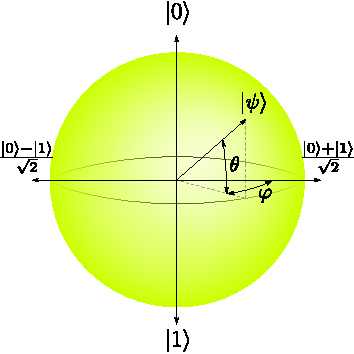
\includegraphics[scale=1]{intro/figs/bloch.pdf}
  \caption{ A quantum state $\ket\psi$ is represented as a point in the surface of the Bloch sphere. The angle theta contains information about the overlap between the state $\ket\psi$ and the basis states $\ket 0$ and $\ket 1$, whereas the angle $\varphi$ describes a phase. \label{fig1:bloch}}
\end{figure}

We will not go into details about quantum computation and quantum algorithms.
%
This is just an example of the powerful capabilities of a quantum computer, but it is not in the scope of this thesis to convince anyone why we need quantum computers and what can they do for us. A quick Google search will already mention some of its applications in internet security, research, etc.
%
We will instead focus on the most essential part of quantum computers: the qubit. A qubit is a quantum bit. It is the analog of a bit in a classic computer but it is not limited to be either in the state 0 or 1. A qubit can be in any quantum superposition of the states $\ket 0$ and $\ket 1$. Qubits are often represented as points in the surface of a sphere: the Bloch sphere. Indeed, any qubit can be expressed as
\begin{align}
\ket{\psi (\theta,\varphi)}  = {}&{} \cos\frac{\theta}{2}\ket 0 + e^{i\varphi} \sin\frac{\theta}{2}\ket 1,
\end{align}
up to an overall phase,
where $\theta$ and $\varphi$ are the polar and azimuthal angles in the Bloch sphere of Fig.~\ref{fig1:bloch}. The states $\ket 0$ and $\ket 1$ denote the north and south poles, respectively, of the sphere.





A qubit is thus a quantum mechanical two-level system, and we need to find a physical implementation of this two-level system if we want to create a quantum computer. When one thinks about two-level quantum systems the first thing that comes to mind is probably the spin of an electron. That is text-book physics. And that is (maybe) what Daniel Loss and David DiVincenzo thought when they wrote their seminal paper on quantum computation using quantum dots~\cite{Loss1998}.


The idea is very simple: If we can localize one electron and manipulate its spin, we can use the spin states $\ket\ua$ and $\ket \da$ as the qubit states. We also need a mechanism to initialize the qubit into any desired quantum state, read out the output state after running a quantum algorithm and we must also be able to couple this qubit to, at least, another qubit to perform two-qubit gates~\cite{DiVincenzo2000a,Nielsen2010}. In Ref.~\cite{Loss1998} the authors address all these issues and propose to localize the electrons in \textit{quantum dots}.



\section{Quantum dots}

\begin{figure}
  \centering
  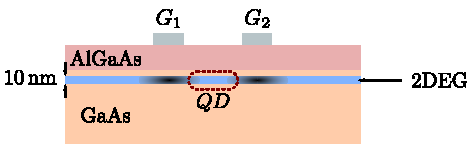
\includegraphics[scale=1]{intro/figs/2deg.pdf}
  \caption{ A 2DEG is formed e.g., close to the interface between a GaAs/AlGaAs heterojunction~\cite{Hanson2007}. It consists of a thin layer ($\sim 10$nm) where electrons can have a high mobility. Top gates ($G_{1}$ and $G_{2}$), lithographically grown, can create a depletion zone in the 2DEG (dark areas), isolating a small region where we can trap one or a few excess electrons (the region enclosed by the dashed red curve). This is a quantum dot.  \label{fig1:2deg}}
\end{figure}

A quantum dot is a potential well that can trap one or a few electrons (or holes). They are typically fabricated in semiconductors, in a two-dimensional electron gas (2DEG). We can think of a 2DEG as a surface in a semiconductor where electrons occupy the conduction band and, thus, can move relatively freely. A 2DEG can be created in Si MOSFETs, in Si/Ge heterostructures, in GaAs/AlGaAs, etc, and in all cases the electrons are confined in a triangular potential along the $z$ direction only, but are unbounded in the $x$-$y$ plane~\cite{Hanson2007,Zwanenburg2013}.


On top of the heterostructure we can put metallic gates. These can be used to apply a localized electric field and create a depletion zone in the 2DEG (see Fig.~\ref{fig1:2deg}). These depletion zones can be engineered to create a whole closed area in the 2DEG where we can trap one or a few electrons. This artificial potential well is a quantum dot.

Once we have a quantum dot we can couple it to a reservoir (by letting electrons tunnel in and out of the quantum dot) and trap one electron. Then we can use the spin of this localized electron for quantum computation.




\section{Making a spin qubit (using quantum dots)}



To understand how a quantum dot-based spin qubit works it is better to see a top view of the device. Fig.~\ref{fig1:2qd} shows a schematic illustration of a system composed of two quantum dots.

\begin{figure}
  \centering
  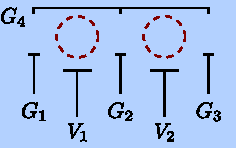
\includegraphics[scale=1]{intro/figs/fig2qd.pdf}
  \caption{ Negative voltages applied to the metallic gates $G_1$, $G_2$, $G_3$ and $G_4$ create a depletion zone in the 2DEG (blue surface). This results in two small isolated islands, the quantum dots, where electrons can be trapped (red circles). The electrochemical potential in the dots can be controlled by the gates $V_1$ and $V_2$. \label{fig1:2qd}}
\end{figure}
The blue surface represents the 2DEG. On top of the device several metallic gates can be individually addressed to create and manipulate the quantum dots: By applying a negative potential on the gates $G_i$, the resulting electric field creates a depletion zone on the 2DEG where electrons are not allowed and a small island where the electrons can be trapped. In Fig.~\ref{fig1:2qd} we show two of such islands, indicated by red dashed circles. These are the quantum dots. We can control the coupling between the two dots by detuning of the gate $G_2$. The gates $G_1$ and $G_3$ can be used to allow electrons in and out of the quantum dots, while the gates $V_1$ and $V_2$ control the electrochemical potential in the dots.

If we now trap one electron in each of the dots we can control its spin with magnetic fields. In fact, with such a simple device, composed of only two quantum dots, it is possible to implement a quantum algorithm~\cite{Watson2018}.

But in this thesis we are not interested in single-spin qubits. The goal of our project is to study decoherence mechanisms in exchange-only spin qubits and mitigate their effects.



\chapter{Statistical Mechanics}
\label{ch:statmech}
\input{statmech}
\chapter{Monte-Carlo Simulations}
\label{ch:MC}
\input{MC}
\chapter{Bose-Einstein Condensates}
\label{ch:BEC}
\input{BEC}
\chapter{Multiband Superconductors}
\label{ch:MBSC}
\input{MBSC}
\bibliographystyle{apsrev4-1}
\bibliography{thesis}
\clearpage
\pagestyle{empty}
\ChTitleVar{\centering\Large\bfseries}
\chapter*{Paper I}
\addcontentsline{toc}{chapter}{Paper I}
\centering \textit{Fluctuation effects in rotating Bose-Einstein condensates with broken
$\mathrm{SU}(2)$and $\mathrm{U}(1)\times\mathrm{U}(1)$ symmetries in the presence of intercomponent
density-density interactions}\\
\bigskip
\centering Physical Review A {\bf 91}, 013605 (2015)
% \clearpage
\cleardoublepage
\includepdf[pages=-]{PaperI.pdf}
\chapter*{Paper II}
\addcontentsline{toc}{chapter}{Paper II}
\centering \textit{Thermal remixing of phase-separated states in two-component bosonic condensates}\\
\bigskip
\centering New Journal of Physics {\bf 17}, 103040 (2015)
\cleardoublepage
\includepdf[pages=2-]{PaperII.pdf}
% \chapter*{Paper III}
% \addcontentsline{toc}{chapter}{Paper III}
% \centering \textit{Paired phase- and density wave states in imbalanced two-dimensional Bose gases}\\
% \bigskip
% \centering Preprint
% \cleardoublepage
% \includepdf[pages=-]{PaperIII.pdf}
\chapter*{Paper III}
\addcontentsline{toc}{chapter}{Paper III}
\centering \textit{Competing interactions in population imbalanced two-component Bose-Einstein
condensates}\\
\bigskip
\centering Preprint
\cleardoublepage
\includepdf[pages=-]{PaperIV.pdf}
\chapter*{Paper IV}
\addcontentsline{toc}{chapter}{Paper IV}
\centering \textit{Current-loops, phase transitions, and the Higgs mechanism in Josephson-coupled
multi-component London superconductors}\\
\bigskip
\centering Preprint (submitted to Phys. Rev. B)
\cleardoublepage
\includepdf[pages=-]{PaperV.pdf}
\end{document}
